%%%%%%%%%%%%%%%%%%%%%%%%%%%%%%%%%%%%%%%%%%%%%%%%%%
%% Layer Overview
%%%%%%%%%%%%%%%%%%%%%%%%%%%%%%%%%%%%%%%%%%%%%%%%%%


%%%%%%%%%%%%%%%%%%%%%%%%%%%%%%%%%%%%%%%%%%%%%%%%%%
%% Subsystem X - Template
%%%%%%%%%%%%%%%%%%%%%%%%%%%%%%%%%%%%%%%%%%%%%%%%%%

% \subsection{Subsystem X}
% Descibe at a high level the purpose and basic design of this subsystem. Is it a piece of hardware, a class, a web service, or something else? Note that each of the subsystem items below are meant to be specific to that subystem and not a repeat of anything discussed above for the overall layer.

% \begin{figure}[h!]
% 	\centering
%  	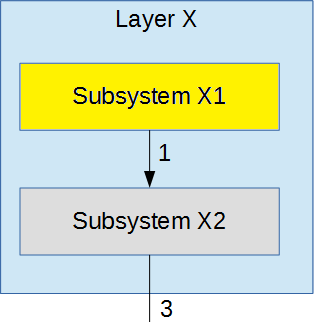
\includegraphics[width=0.60\textwidth]{images/subsystem}
%  \caption{Example subsystem description diagram}
% \end{figure}

% \subsubsection{Subsystem Hardware}
% A description of any involved hardware components for the subsystem.

% \subsubsection{Subsystem Operating System}
% A description of any operating systems required by the subsystem.

% \subsubsection{Subsystem Software Dependencies}
% A description of any software dependencies (libraries, frameworks, design software for mechanical parts or circuits, etc) required by the subsystem.

% \subsubsection{Subsystem Programming Languages}
% A description of any programming languages used by the subsystem.

% \subsubsection{Subsystem Data Structures}
% A description of any classes or other data structures that are worth discussing for the subsystem. For example, data being transmitted from a microcontroller to a PC via USB should be first be assembled into packets. What is the structure of the packets?

% \subsubsection{Subsystem Data Processing}
% A description of any algorithms or processing strategies that are worth discussing for the subsystem. If you are implementing a well-known algorithm, list it. If it is something unique to this project, discuss it in greater detail.



The Pathfinding Subsystem controls the rover's movement, by utilizing the rover's LIDAR to create a map of the terrain. The subsystem will than create a costmap grid, and than applying an A* pathfinding algorithm to find the most efficient and safest path.

\subsection{Navigation}
The Navigation system is a core component responsible for guiding the rover through its environment safely and efficiently. It combines sensor input, mapping, localization, and path planning to enable autonomous movement. Using real-time data from perception subsystems, the navigation system constructs a map of the surroundings, determines the rover's position within that map, and plans feasible routes to target destinations. It continuously updates the robot's trajectory to avoid obstacles and adapt to changes in the environment, ensuring smooth and collision-free traversal. This system is tightly integrated with motion control and localization components to maintain accurate positioning and responsive movement.

\begin{figure}[h!]
	\centering
 	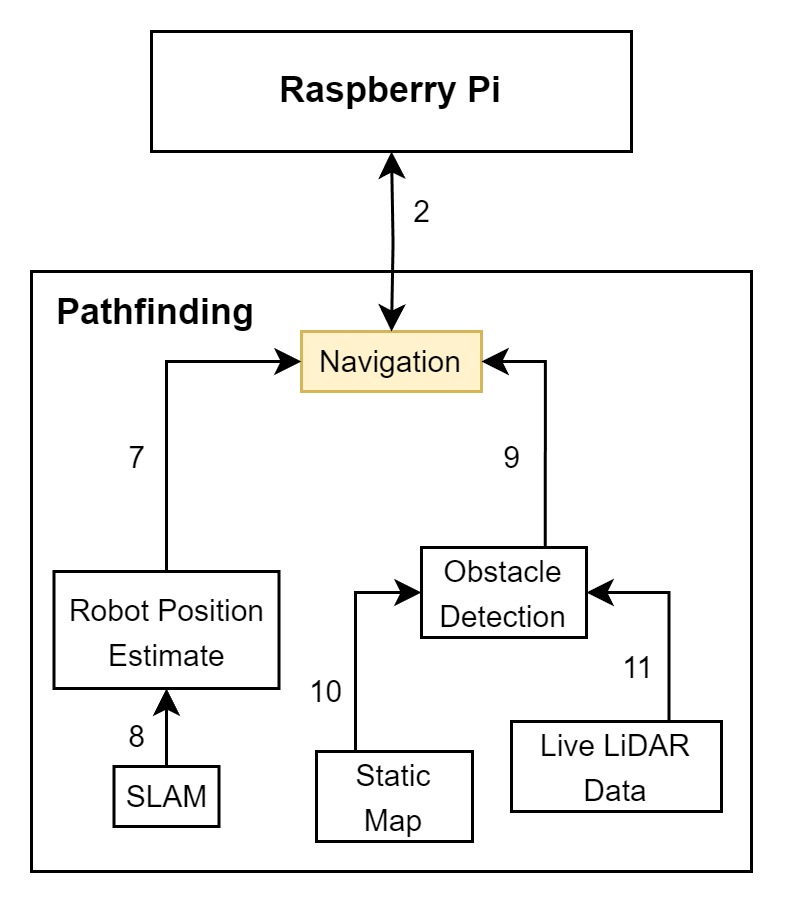
\includegraphics[width=0.60\textwidth]{images/pathfinding/navigation.jpg}
 \caption{Pathfinding Layer - LIDAR Subsystem}
\end{figure}


\subsubsection{Subsystem Hardware}
Slamtec RPLIDAR A1 - 360-degree laser range scanner. With a maximum range of 100 meters and a sampling frequency of a little over 2500 samples a second, measures distances and angles to create a 2D cloud point representation of the surroundings.

\subsubsection{Subsystem Operating System}
The navigation subsystem will be run on ROS2 Jazzy which requires Ubuntu 24.04 (Noble Numbat) or higher for compatibility. 

\subsubsection{Subsystem Dependencies}
The Navigation Subsystem uses Nav2 and ROS2 to develop the pathfinding algorithm and design the path for the rover to follow, and ROS2 to manage the robot's movements.

\subsubsection{Subsystem Programming Languages}
Nav2 is primarily implemented in C++ to ensure optimal compatibility with ROS2, which is also C++-
based. However, it also provides a Python API for additional flexibility.
\subsubsection{Subsystem Data Structures}
The pathfinding subsystem employs the A* algorithm due to its ability to determine the most optimal
path while maintaining lower computational overhead compared to alternative pathfinding methods.
\subsubsection{Subsystem Data Processing}
The pathfinding subsystem employs the A* algorithm due to its ability to determine the most optimal path while maintaining lower computational overhead compared to alternative pathfinding methods. (such as Djikstra, BFS)

\newpage

\subsection{Obstacle Detection}
The Obstacle Detection subsystem leverages the costmap generated by the Grid Management Subsystem to assess the robot's environment. It assigns a numerical value to each grid cell based on the proximity of surrounding objects, with higher values indicating closer objects and lower values representing areas free from obstacles.

\begin{figure}[h!]
	\centering
 	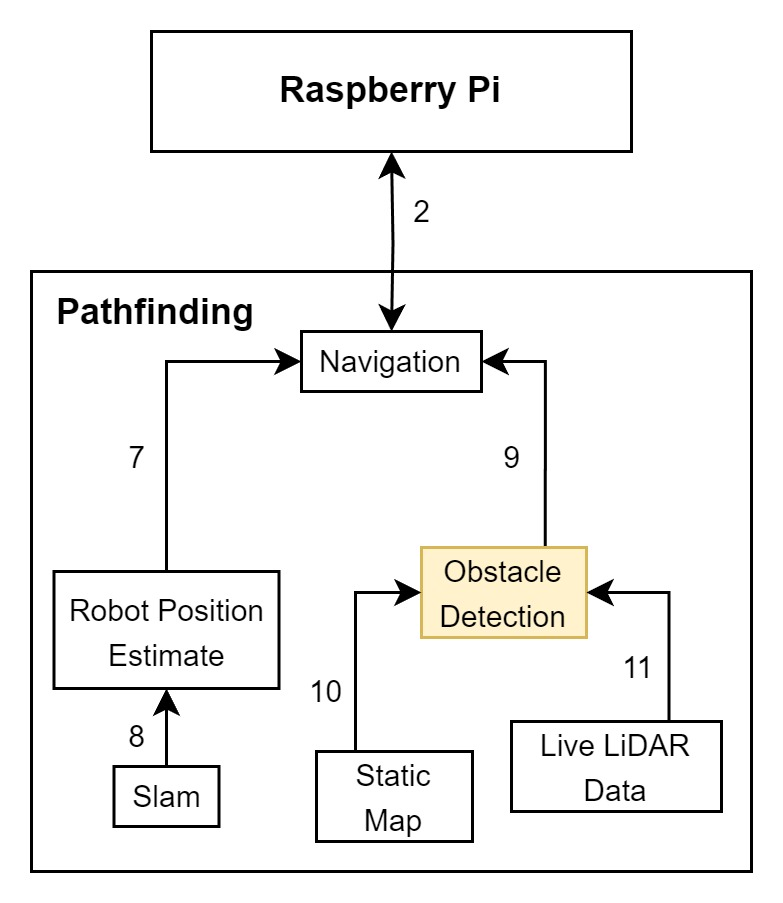
\includegraphics[width=0.60\textwidth]{images/pathfinding/obstacledetection.jpg}
 \caption{Pathfinding Layer - Navigation Subsystem}
\end{figure}

%\subsubsection{Subsystem Hardware}
%The navigation software will be housed on the Raspberry Pi 5.
\subsubsection{Subsystem Operating System}
%A description of any operating systems required by the subsystem.
ROS2 Jazzy requires Ubuntu 24.04 (Noble Numbat) or higher for compatibility.
\subsubsection{Subsystem Software Dependencies}
%A description of any software dependencies (libraries, frameworks, design software for mechanical parts or circuits, etc) required by the subsystem.
The Obstacle Detection Subsystem uses Nav2 to develop the pathfinding algorithm and design the path for the rover to follow, and ROS2 to manage the robot's movements.

\subsubsection{Subsystem Programming Languages}
%A description of any programming languages used by %the subsystem.
Nav2 is primarily in C++, so it can better configure with ROS2 which is also in C++, but Nav2 does allow for a Python API.

\newpage

\subsection{Static Map}
The Static Map subsystem provides foundational spatial information for the rover's autonomous navigation. It consists of a pre-built occupancy grid defines known obstacles and traversable areas within a fixed environment, creating a costmap. In a ROS 2 and Nav2-based system, this map is loaded at runtime and used by the global planner to calculate optimal paths from the rover's current position to a designated goal. The static map enables efficient pathfinding by offering a reliable reference frame for localization and route generation.

\begin{figure}[h!]
	\centering
 	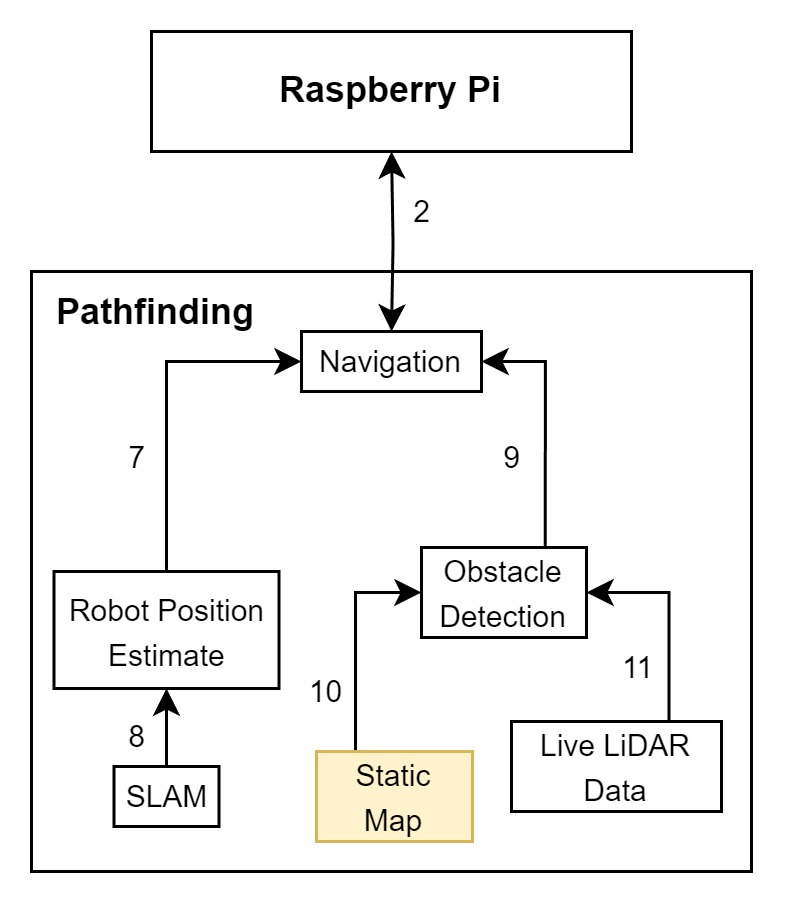
\includegraphics[width=0.60\textwidth]{images/pathfinding/staticmap.jpg}
 \caption{Pathfinding Layer - Static Map Subsystem}
\end{figure}


%\subsubsection{Subsystem Hardware}
%The Grid Management runs on Ros2 Jazzy which will be stored on the Raspberry Pi 5.
%\subsubsection{Subsystem Operating System}
%The Grid Management Subsystem will operate on ROS2 Jazzy, which requires Ubuntu 24.04 or later
\subsubsection{Subsystem Operating System}
Our Roam\_Bot utilizes a Slamtec RPLIDAR A1 - 360 Laser Range Scanner to create the static map
\subsubsection{Subsystem Software Dependencies}
The Static Map Subsystem uses Nav2 to to create the static map.
% \subsubsection{Subsystem Data Structures}

\newpage

\subsection{Live LiDAR Data}

The Live LiDAR Data subsystem provides real-time environmental awareness for the rover's navigation stack.  As the LIDAR sensor continuously scans the surroundings, it generates a dynamic stream of range measurements that are processed into a real-time occupancy grid.


\begin{figure}[h!]
	\centering
 	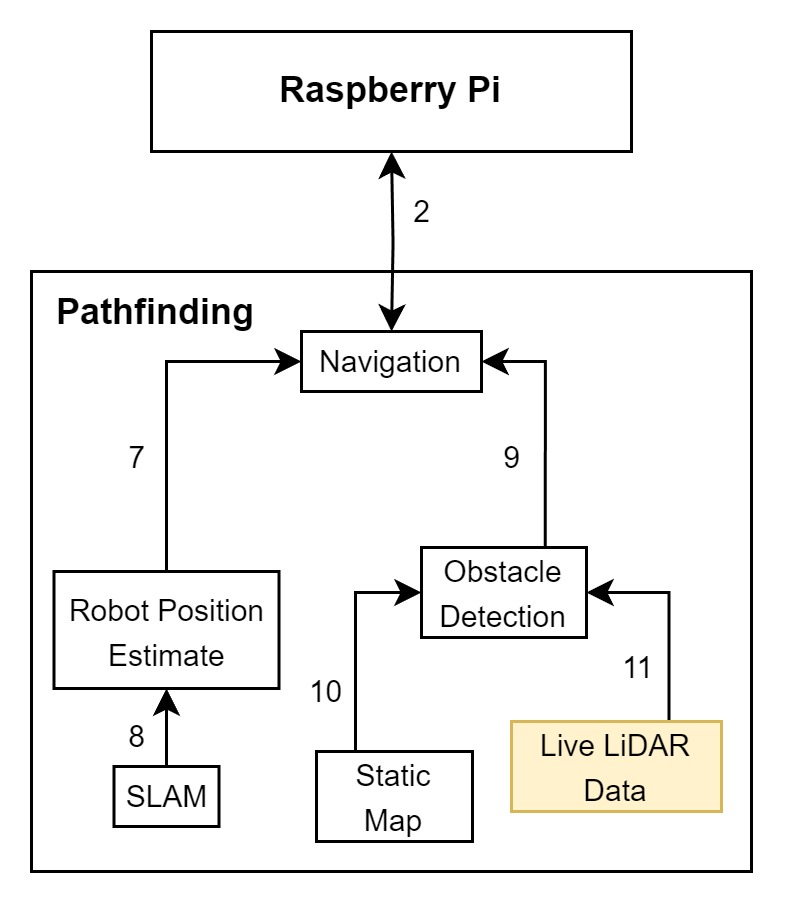
\includegraphics[width=0.60\textwidth]{images/pathfinding/livelidardata.jpg}
 \caption{Pathfinding Layer - Live LiDAR Data Subsystem}
\end{figure}

\subsubsection{Subsystem Hardware}
Our Roam\_Bot utilizes a Slamtec RPLIDAR A1 - 360 Laser Range Scanner. 


\subsubsection{Subsystem Operating System}
%A description of any operating systems required by the subsystem.
ROS2 Jazzy requires Ubuntu 24.04 (Noble Numbat) or higher for compatibility.

\newpage
\subsection{Robot Position Estimate}
% Descibe at a high level the purpose and basic design of this subsystem. Is it a piece of hardware, a class, a web service, or something else? Note that each of the subsystem items below are meant to be specific to that subystem and not a repeat of anything discussed above for the overall layer.
The robot position estimate subsystem is a software component responsible for determining the rover's location and orientation within its environment. It operates as part of the localization layer and integrates data from odometry, and LIDAR. The subsystem continuously fuses sensor inputs using probabilistic filtering techniques to maintain a stable and consistent position estimate, which is critical for navigation, path planning, and obstacle avoidance.

\begin{figure}[h!]
 	\centering
  	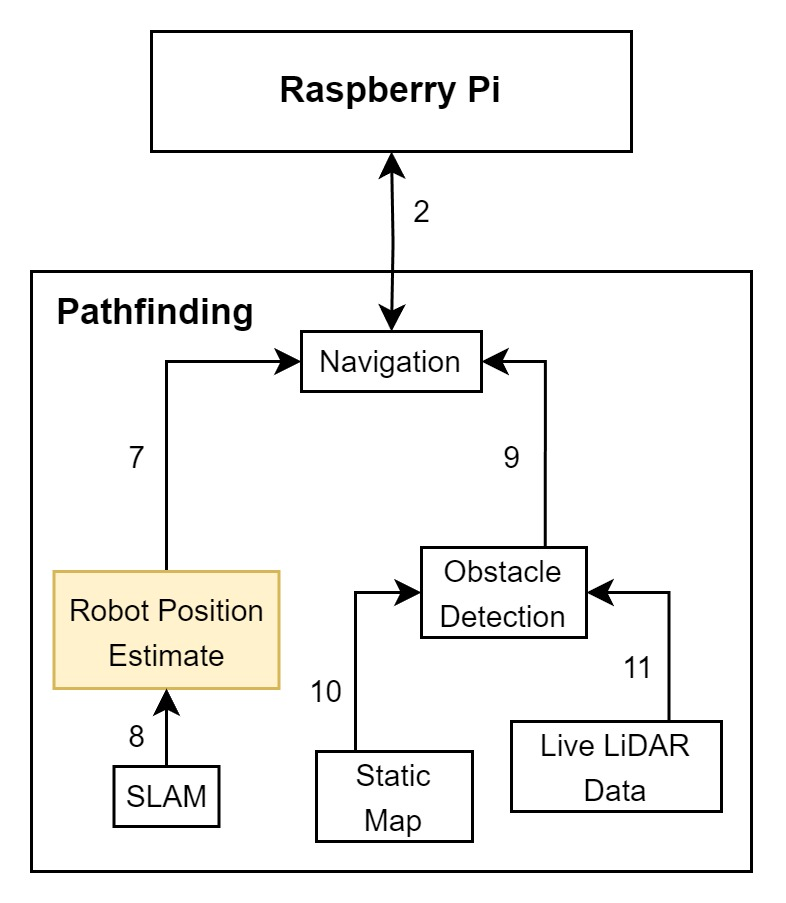
\includegraphics[width=0.60\textwidth]{images/pathfinding/robotpositionestimate.jpg}
  \caption{Pathfinding Layer - Robot Position Estimate}
 \end{figure}

 \subsubsection{Subsystem Hardware}
To create a position estimate for our Roam\_Bot we utilize our Slamtec RPLIDAR A1. 

\subsubsection{Subsystem Operating System}
ROS2 Jazzy requires Ubuntu 24.04 (Noble Numbat) or higher for compatibility.

\subsubsection{Subsystem Software Dependencies}
The Robot Position Estimate is calculated using ROS2 Jazzy and Nav2

\subsubsection{Subsystem Programming Languages}
the Robot Position Estimate is programmed in C++.

\newpage
\subsection{SLAM}
% Descibe at a high level the purpose and basic design of this subsystem. Is it a piece of hardware, a class, a web service, or something else? Note that each of the subsystem items below are meant to be specific to that subystem and not a repeat of anything discussed above for the overall layer.
The SLAM (Simultaneous Localization and Mapping) subsystem is a software module that enables the rover to navigate unknown environments by building a map while simultaneously estimating its position within it. As the robot moves, SLAM compares incoming sensor data to previous scans to update both its map and its own position. 

\begin{figure}[h!]
	\centering
 	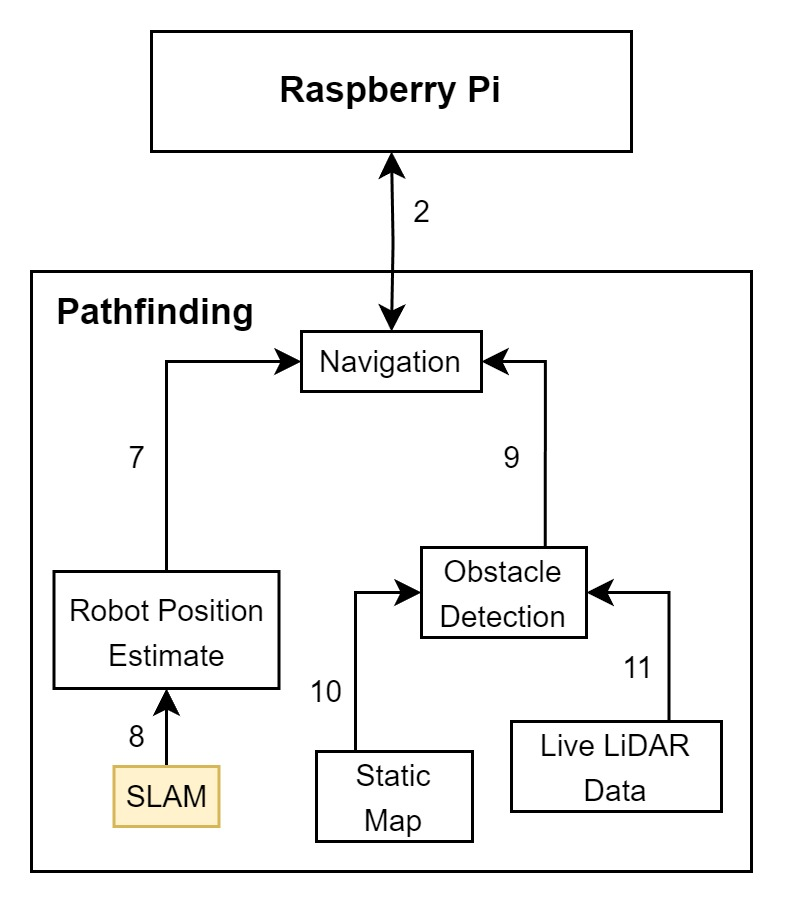
\includegraphics[width=0.60\textwidth]{images/pathfinding/slam.jpg}
 \caption{Pathfinding Layer - SLAM}
\end{figure}

\subsubsection{Subsystem Hardware}
SLAM relies on the SlamTec Lidar to derive the robot position estimate and map the floor,

\subsubsection{Subsystem Operating System}
% A description of any operating systems required by the subsystem.
ROS2 Jazzy requires Ubuntu 24.04 (Noble Numbat) or higher for compatibility.

\subsubsection{Subsystem Software Dependencies}
SLAM is calculated using ROS2 Jazzy and Nav2

\subsubsection{Subsystem Programming Languages}
% A description of any programming languages used by the subsystem.
Nav2 is primarily in C++, so it can better configure with ROS2 which is also in C++, but Nav2 does allow for a Python API.